\documentclass[12pt,oneside,a4paper,reqno]{report}
\usepackage[english]{babel}
\usepackage[utf8x]{vietnam}
% package for including graphics with figure-environment
\usepackage{graphicx}
\usepackage{amsmath,amssymb,exscale,eucal,amsthm, mathrsfs}

%\DeclareMathSizes{12}{15}{9}{9}
\usepackage[table,xcdraw]{xcolor}
\usepackage{tabularx}
\usepackage{longtable}

\usepackage[portrait, top=3.5 cm, bottom=3cm, left=3.5cm, right=2cm] {geometry}
% colors for hyperlinks
% colored borders (false) colored text (true)
\usepackage{wrapfig}
\usepackage{color}
%\usepackage{caption}
% package for bibliography
%\usepackage[round, sort, numbers]{natbib}
% package for header
 

\setlength{\baselineskip}{16truept}
%\renewcommand{\baselinestretch}{1.45}
%%
\renewcommand{\baselinestretch}{1.5}%%đổi về 1.5
%\renewcommand{\baselineskip{1.5}}


\usepackage{enumitem}
%===========thư viện cho header và footer==================
\usepackage{fancyhdr}
\pagestyle{fancy}
%====================================================
\rhead{\textbf{\emph{Đào Tuấn Anh, Vũ Thanh Tùng - KSTN TOÁN TIN K57}}}
\lhead{}
\lfoot{\textbf{Tìm hiểu về SNMP và công cụ giám sát mạng}}
\cfoot{}
\rfoot{\thepage}
\renewcommand{\headrulewidth}{0.4pt}
\renewcommand{\footrulewidth}{0.4pt}
%=====================================================


\begin{document}
\begin{large}

	\begin{titlepage}
\begin{longtable}{p{4cm}p{2cm}p{7cm}}
\centerline{\bf TRƯỜNG ĐẠI HỌC BÁCH KHOA HÀ NỘI}\\
\centerline{\bf VIỆN TOÁN ỨNG DỤNG VÀ TIN HỌC}\\
\centerline{\bf -----------------*-----------------}\\
\end{longtable}

\vspace*{1 cm}

\begin{center}

\includegraphics[width=0.1\textwidth]{images/bkhn.jpg}
\end{center}

\vspace*{1cm}
\centerline{\large\bf BÁO CÁO BÀI TẬP LỚN}

\centerline{\large\bf Môn: Thiết kế, cài đặt và quản trị mạng máy tính}
	
\vspace{1cm}
\centerline{\Large\bf  Đề tài: Tìm hiểu về SNMP và công cụ giám sát mạng Cacti}


\vspace*{1cm}

\begin{center}

$
\begin{array}{llll}
\text{Giảng viên hướng dẫn }&\text{:}
&\text{ThS.  Nguyễn Tuấn Dũng}
\\
\text{Sinh viên thực hiện }&\text{:}
&\text{Đào Tuấn Anh (MSSV: 20121178)}
\\
&\text{:}
&\text{Vũ Thanh Tùng (MSSV: 20124917)}
\\
\text{Lớp }&\text{:}&\text{KSTN TOÁN TIN K57}

\end{array}
$

\end{center}

\vfill
\centerline{\large\bf Hà Nội -- Năm 2016}
\vspace*{0.3cm}
\end{titlepage}
	
\newpage
\tableofcontents
\newpage
	

%%
\newpage
\vspace*{0.2cm}
\centerline{\Large\bf LỜI MỞ ĐẦU}
\vspace*{0.5cm}
\addcontentsline{toc}{chapter}{\bf LỜI MỞ ĐẦU}

Sự phát triển không ngừng nghỉ của công nghệ thông tin đã tạo ra những thay đổi lớn trong cơ sở hạ tầng, lực lượng sản xuất, tính chất lao động, cấu trúc kinh tế và cả cách thức quản lý trong các lĩnh vực của xã hội. Một trong những yếu tố quyết định trong đó, cũng là một nhu cầu tất yếu là việc trao đổi thông tin giữa các thiết bị thông qua mạng máy tính. Sự tăng nhanh về kích cỡ của các hệ thống mạng đã và đang đưa ra thách thức không nhỏ cho người quản trị trong việc theo dõi và quản lý.

Do đó, các hệ thống giám sát an toàn mạng ra đời, đóng vai trò quan trọng, không thể thiếu trong hạ tầng công nghệ thông tin của các cơ quan, đơn vị, tổ chức. Hệ thống này cho phép thu thập, chuẩn hóa, lưu trữ và phân tích tương quan toàn bộ các sự kiện được sinh ra trong hệ thống mạng của tổ chức. Từ đó người quản trị có thể dễ dàng đưa ra phân tích, thống kê, cảnh báo, nắm bắt thực trạng tài nguyên, khắc phục sự cố, đồng thời ngăn chặn sớm các mối nguy hiểm cho hệ thống.

Nội dung dưới đây có đề cập đến giao thức quản lý mạng SNMP (Simple Network Management Protocol). SNMP là một tập hợp các giao thức không chỉ cho phép kiểm tra các thiết bị mạng như router, switch hay server có đang vận hành mà còn hỗ trợ vận hành các thiết bị này một cách tối ưu, ngoài ra SNMP còn cho phép quản lý các thiết bị mạng từ xa. Bên cạnh đó, báo cáo còn đề cập đến Cacti, một hệ thống quản lý tài nguyên mạng mã nguồn mở. Phần mềm này đáp ứng nhu cầu quản lý mạng một cách toàn diện với nhiều tính năng linh hoạt vượt trội.

Em xin chân thành cảm ơn thầy Nguyễn Tuấn Dũng đã tận tình truyền đạt kiến thức trong suốt môn học. Tuy nhiên trong khoảng thời gian cho phép, việc nghiên cứu và trình bày không thể tránh khỏi nhầm lẫn thiếu sót, em mong nhận được sự giúp đỡ đóng góp của thầy cô và bạn bè để bài báo cáo được hoàn thiện hơn.



%---------------------------------------------------
%---------------------------------------------------
\chapter{GIAO THỨC SNMP VÀ CÁC VẤN ĐỀ LIÊN QUAN}
\section{Tổng quan về quản lý hệ thống mạng}
\subsection{Khái niệm quản lý hệ thống mạng}
Quản lý hệ thống mạng là việc thực hiện tập hợp các chức năng cần thiết cho việc kiểm soát, lập kế hoạch, phân bổ, triển khai, phối hợp và giám sát các nguồn tài nguyên trong hệ thống. Nó thường được áp dụng cho các mạng quy mô lớn như mạng máy tính và mạng viễn thông, đề cập đến việc duy trì và quản trị mạng ở cấp cao nhất.
\subsection{Khái niệm giám sát mạng}
Giám sát mạng là việc sử dụng một hệ thống liên tục theo dõi hoạt động của một mạng máy tính, thông báo ngay lập tức và cho phép người quản trị mạng biết trong trường hợp xảy ra sự cố ảnh hưởng đến tốc độ hoặc lỗi mạng.

Giám sát mạng là một phần trong quản lý hệ thống mạng.

Một hệ thống giám sát mạng sẽ theo dõi hệ thống mạng gây ra bởi quá tải hay máy chủ bị sập, bởi các kết nối trong mạng hoặc từ các thiết bị khác. Các thông số đánh giá thường gặp là thời gian phản hồi, hiệu lực và thời gian vận hành tối thiểu trung bình (uptime). Ngoài ra còn có các thông số phổ biến khác như độ ổn định hay độ tin cậy.

Ví dụ, để kiểm tra một máy chủ Web, phần mềm giám sát sẽ gửi đều đặn các truy vấn HTTP để lấy nội dung trang web. Ở các máy chủ thư, các gói tin kiểm tra sẽ được gửi đều đặn thông qua SMTP, và nhận lại qua IMAP hoặc POP3.
\subsection{Hai phương thức giám sát mạng: Poll và Alert}
Hai giao thức giám sát “Poll” và “Alert” là 2 phương thức cơ bản của các kỹ thuật giám sát hệ thống, nhiều phần mềm và giao thức được xây dựng dựa trên 2 phương thức này, trong đó có SNMP.

\textbf{Phương thức Poll}

\begin{center}
	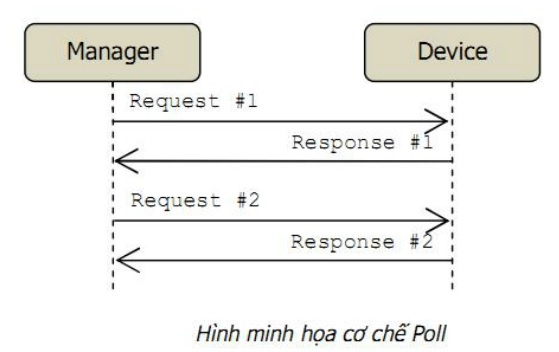
\includegraphics[scale=0.5]{images/poll.jpg}
\end{center}

Nguyên tắc hoạt động: Trung tâm giám sát (manager) sẽ thường xuyên hỏi thông tin của các thiết bị cần giám sát (device). Nếu manager không hỏi thì device không trả lời, nếu manager hỏi thì device trả lời. Bằng cách hỏi thường xuyên, manager sẽ luôn cập nhật được thông tin mới nhất từ device.

\textbf{Phương thức Alert}
\begin{center}
	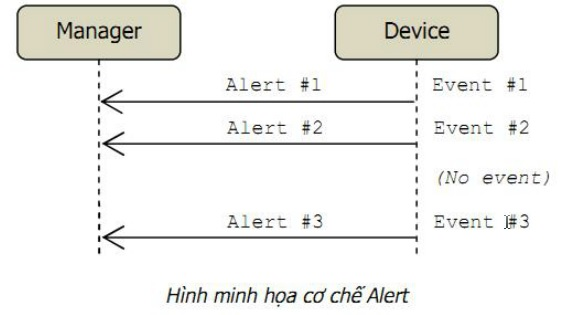
\includegraphics[scale=0.5]{images/alert.jpg}
\end{center}
Nguyên tắc hoạt động: Mỗi khi trong device xảy ra một sự kiện (event) nào đó thì device sẽ tự động gửi thông báo cho Manager, gọi là alert. Manager không hỏi thông tin định kỳ từ device.

Device chỉ gửi những thông báo mang tính sự kiện chứ không gửi những thông tin thường xuyên thay đổi, nó cũng sẽ không gửi Alert nếu chẳng có sự kiện gì xảy ra. Chẳng hạn khi một port down/up thì Device sẽ gửi cảnh báo, còn tổng số byte truyền qua port đó sẽ không được Device gửi đi vì đó là thông tin thường xuyên thay đổi. Muốn lấy những thông tin thường xuyên thay đổi thì Manager phải chủ động đi hỏi device, tức là phải thực hiện phương thức Poll.

\textbf{So sánh 2 phương thức Poll và Alert}

Hai phương thức Poll và Alert là hoàn toàn khác nhau về cơ chế. Một ứng dụng giám sát có thể sử dụng Poll hoặc Alert, hoặc cả hai, tùy vào yêu cầu cụ thể trong thực tế.

Bảng sau so sánh những điểm khác biệt của 2 phương thức:
\newpage
\begin{longtable}{|p{8cm}|p{8cm}|}
\hline
\rowcolor[HTML]{EFEFEF} 
\multicolumn{1}{|c|}{\cellcolor[HTML]{EFEFEF}\textbf{POLL}}                                                                                                                                                                                                    & \multicolumn{1}{c|}{\cellcolor[HTML]{EFEFEF}\textbf{ALERT}}                                                                                                                                                                                   \\ \hline
Có thể chủ động lấy những thông tin cần thiết từ các đối tượng mình quan tâm, không cần lấy những thông tin không cần thiết từ những nguồn không quan tâm.                                                                                                     & Tất cả những event xảy ra đều được gửi về Manager. Manager phải có cơ chế lọc những event cần thiết, hoặc Device phải thiết lập được cơ chế chỉ gửi những event cần thiết.                                                                    \\ \hline
Có thể lập bảng trạng thái tất cả các thông tin của Device sau khi poll qua một lượt các thông tin đó.                                                                                                                                                         & Nếu không có event gì xảy ra thì Manager không biết được trạng thái của Device.                                                                                                                                                               \\ \hline
Trong trường hợp đường truyền giữa Manager và Device xảy ra gián đoạn và Device có sự thay đổi, thì Manager sẽ không thể cập nhật. Tuy nhiên khi đường truyền thông suốt trở lại thì Manager sẽ cập nhật được thông tin mới nhất do nó luôn luôn poll định kỳ. & Khi đường truyền gián đoạn và Device có sự thay đổi thì nó vẫn gửi Alert cho Manager, nhưng Alert này sẽ không thể đến được Manager. Sau đó mặc dù đường truyền có thông suốt trở lại thì Manager vẫn không thể biết được những gì đã xảy ra. \\ \hline
Chỉ cần cài đặt tại Manager để trỏ đến tất cả các Device. Có thể dễ dàng thay đổi một Manager khác.                                                                                                                                                            & Phải cài đặt từng Device để trỏ đến Manager. Khi thay đổi Manager thì phải cài đặt lại trên tất cả Device để trỏ về Manager mới.                                                                                                              \\ \hline
Nếu tần suất poll thấp, thời gian chờ giữa 2 chu kỳ poll dài sẽ làm Manager chậm cập nhật các thay đổi của Device. Nghĩa là nếu thông tin Device đã thay đổi nhưng vẫn chưa đến lượt poll kế tiếp thì Manager vẫn giữ thông tin cũ.                            & Ngay khi có sự kiện xảy ra thì Device sẽ gửi Alert đến Manager, do đó Manager luôn luôn có thông tin mới nhất tức thời.                                                                                                                       \\ \hline
Có thể bỏ sót các sự kiện : khi Device có thay đổi, sau đó thay đổi trở lại như ban đâu trước khi đến lượt poll kế tiếp thì Manager sẽ không phát hiện được.                                                                                                   & Manager sẽ được thông báo mỗi khi có sự kiện xảy ra ở Device, do đó Manager không bỏ sót bất kỳ sự kiện nào.                                                                                                                                  \\ \hline
\end{longtable}

\section{Giao thức quản lý mạng SNMP (Simple Network Management Protocol)}
\subsection{Giới thiệu giao thức SNMP}
SNMP (viết tắt từ tiếng Anh: Simple Network Management Protocol) là {\it giao thức quản lý mạng đơn giản}.

Rõ thêm, giao thức là một tập hợp các thủ tục mà các bên tham gia cần tuân theo để có thể giao tiếp được với nhau. Trong lĩnh vực thông tin, một giao thức quy định cấu trúc, định dạng của dòng dữ liệu trao đổi với nhau và quy định trình tự, thủ tục để trao đổi dòng dữ liệu đó. Nếu một bên tham gia gửi dữ liệu không đúng định dạng hoặc không theo trình tự thì các bên khác sẽ không hiểu hoặc từ chối trao đổi thông tin. SNMP là một giao thức, do đó nó có những quy định riêng mà các thành phần trong mạng phải tuân theo. Một thiết bị hiểu được và hoạt động tuân theo giao thức SNMP được gọi là “có hỗ trợ SNMP” (SNMP supported) hoặc “tương thích SNMP” (SNMP compartible).

SNMP dùng để quản lý mạng, nghĩa là nó được thiết kế để chạy trên nền TCP/IP và quản lý các thiết bị có kết nối mạng TCP/IP. Các thiết bị mạng không nhất thiết phải là máy tính mà có thể là switch, router, firewall, ADSL gateway, và cả một số phần mềm cho phép quản trị bằng SNMP.

Giao thức SNMP sẽ giải quyết được các bài toán về giám sát tài nguyên máy chủ; giám sát hiệu năng, lưu lượng trên các thiết bị mạng; hệ thống cảnh báo sự cố tức thời.

SNMP là giao thức đơn giản, do nó được thiết kế đơn giản trong cấu trúc bản tin và thủ tục hoạt động, bảo mật. Sử dụng phần mềm SNMP, người quản trị mạng có thể quản lý, giám sát tập trung từ xa toàn mạng của mình.
\subsection{Ưu nhược điểm của giao thức SNMP}

\textbf{Ưu điểm của thiết kế SNMP}

+) SNMP được thiết kế đơn giản hóa quá trình quản lý các thành phần trong mạng. Nhờ đó các phần mềm SNMP có thể được phát triển nhanh và tốn ít chi phí.

+) SNMP được thiết kế có thể mở rộng các chức năng quản lý, giám sát. Không có giới hạn rằng SNMP có thể quản lý được cái gì. Khi có một thiết bị mới với các thuộc tính, tính năng mới thì người ta có thể thiết kế “custom” SNMP để phục vụ cho riêng mình.

+) SNMP được thiết kế có thể hoạt động độc lập với các kiến trúc và cơ chế của các thiết bị hỗ trợ SNMP. Các thiết bị khác nhau có hoạt động khác nhau nhưng đáp ứng SNMP là giống nhau.

\textbf{Nhược điểm của SNMP}

+) Làm tăng lưu lượng đáng kể.

+) Không có sự điều khiển tổng hợp của nhiều nơi quản lý.
\subsection{Các phiên bản giao thức SNMP}
SNMP có 4 phiên bản: SNMPvl, SNMPv2c, SNMPv2u và SNMPv3. Các phiên bản này khác nhau một chút ớ định dạng bán tin và phương thức hoạt động. Hiện tại SNMPvl là phổ biến nhất do có nhiều thiết bị tương thích nhất và có nhiều phần mềm hồ trợ nhất. Trong khi đó chỉ có một số thiết bị và phần mềm hỗ trợ SNMPv3.

- \textbf{Phiên bản SNMPv1}: phiên bản đầu tiên của SNMP, có 5 phương thức Get, GetNext, Set, Response, Trap. 

\begin{itemize}

\item GetRequest: Bản tin GetRequest được manager gửi đến agent để lấy một thông tin nào đó. Trong GetRequest có chứa ID của object muốn lấy. Ví dụ: Muốn lấy thông tin tên của Device1 thì manager gửi bản tin GetRequest ID=1.3.6.1.2.1.1.5 đến Device1, tiến trình SNMP agent trên Device1 sẽ nhận được bản tin và tạo bản tin trả lời. Trong một bản tin GetRequest có thể chứa nhiều OID, nghĩa là dùng một GetRequest có thể lấy về cùng lúc nhiều thông tin.

\item GetNextRequest: Bản tin GetNextRequest cũng dùng để lấy thông tin và cũng có chứa OID, tuy nhiên nó dùng để lấy thông tin của object nằm kế tiếp object được chỉ ra trong bản tin. Chúng ta đã biết khi đọc qua những phần trên: một MIB bao gồm nhiều OID được sắp xếp thứ tự nhưng không liên tục, nếu biết một OID thì không xác định được OID kế tiếp. Do đó ta cần GetNextRequest để lấy về giá trị của OID kế tiếp. Nếu thực hiện GetNextRequest liên tục thì ta sẽ lấy được toàn bộ thông tin của agent.

\item SetRequest: Bản tin SetRequest được manager gửi cho agent để thiết lập giá trị cho một object nào đó. Ví dụ: Có thể đặt lại tên của một máy tính hay router bằng phần mềm SNMP manager, bằng cách gửi bản tin SetRequest có OID là 1.3.6.1.2.1.1.5.0 (sysName.0) và có giá trị là tên mới cần đặt.

\item GetResponse: Mỗi khi SNMP agent nhận được các bản tin GetRequest, GetNextRequest hay SetRequest thì nó sẽ gửi lại bản tin GetResponse để trả lời. Trong bản tin GetResponse có chứa OID của object được request và giá trị của object đó. 

\item Trap: Bản tin Trap được agent tự động gửi cho manager mỗi khi có sự kiện xảy ra bên trong agent, các sự kiện này không phải là các hoạt động thường xuyên của agent mà là các sự kiện mang tính biến cố. Ví dụ: Khi có một port down, khi có một người dùng login không thành công, hoặc khi thiết bị khởi động lại, agent sẽ gửi trap cho manager. Tuy nhiên không phải mọi biến cố đều được agent gửi trap, cũng không phải mọi agent đều gửi trap khi xảy ra cùng một biến cố. Việc agent gửi hay không gửi trap cho biến cố nào là do hãng sản xuất device/agent quy định.
\end{itemize}

\begin{center}
	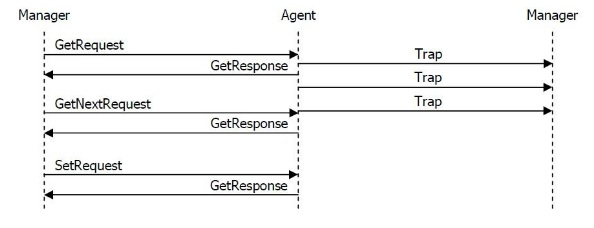
\includegraphics[scale=1]{images/snmpv1.jpg}\\
	Các phương thức trong SNMPv1
\end{center}

- \textbf{Phiên bản SNMPv2}: SNMPv2 tích hợp khả năng liên điều hành từ manager tới manager và hai đơn vị dữ liệu giao thức mới. Khả năng liên kết điều hành manager- manager cho phép SNMP hỗ trợ quản lí mạng phân tán trong một trạm và gửi báo cáo tới một trạm khác. Hai đơn vị dữ liệu giao thức PDU (Protocol Data Unit) là GetbulkRequest và InformRequest. Các PDU này liên quan tới xử lý lỗi và khả năng đếm của SNMPv2. Khả năng đếm trong SNMPv2 sử dụng bộ đếm 64 bit (hoặc 32) để duy trì trạng thái của các liên kết và giao diện.

\textbf{MIB cho SNMPv2}: MIB trong SNMPv2 định nghĩa các đối tượng mô tả tác động của một phần tử SNMPv2.MIB gồm 3 nhóm: 

+ Nhóm hệ thống (System group): là một mở rộng của nhóm system trong MIB-II gốc, bao gồm một nhóm các đối tượng cho phép một Agent SNMPv2 mô tả các đối tượng tài nguyên của nó. 

+ Nhóm SNMP (SNMP group): một cải tiến của nhóm SNMP trong MIB-II gốc, bao gồm các đối tượng cung cấp các công cụ cơ bản cho hoạt động giao thức. 

+ Nhóm các đối tượng MIB (MIB objects group): một tập hợp các đối tượng liên quan đến các SNMPv2-trap PDU và cho phép một vài phần tử SNMPv2 cùng hoạt động, thực hiện như trạm quản trị, phối hợp việc sử dụng của chúng trong toán tử Set của SNMPv2 

Nhóm hệ thống: nhóm system định nghĩa trong SNMPv2 giống trong MIB-II và bổ sung một vài đối tượng mới. 

Nhóm SNMP: Nhóm này gần giống như nhóm SNMP đươc định nghĩa trong MIB-II nhưng có thêm một số đối tượng mới và loại bỏ một số đối tượng ban đầu. Nhóm SNMP chứa một vài thông tin lưu lượng cơ bản liên quan đến toán tử SNMPv2 và chỉ cómột trong các đối tượng là bộ đệm chỉ đọc 32-bit.

Nhóm đối tượng MIB: Nhóm các đối tượng MIB chứa các đối tượng thích hợp thêm vào việc điều khiển các đối tượng MIB. 

\newpage

\textbf{Cấu trúc bản tin SNMPv2}: 

\begin{center}
	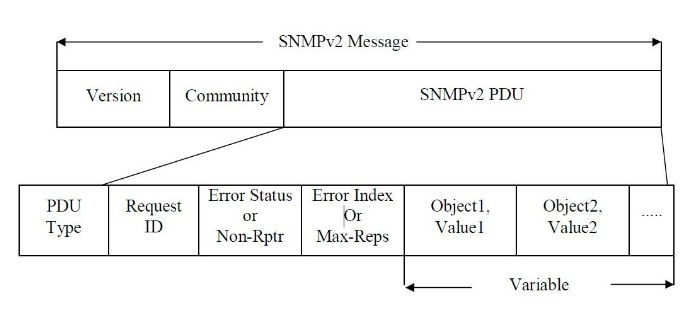
\includegraphics[scale=0.7]{images/snmpv2.jpg}\\
	Cấu trúc bản tin SNMPv2
\end{center}

Trường phiên bản (Version) thể hiện phiên bản của giao thức SNMPv2. 

Trường Community là một chuỗi password xác nhận cho cả tiến trình lấy và thay đổi dữ liệu. SNMP PDU chứa kiểu điều hành (get, set), yêu cầu đáp ứng (cùng số thứ tự với bản tin gửi đi) - cho phép người điều hành gửi đồng thời nhiều bản tin. Biến ghép gồm các thiết bị được đặc tả trong RFC 2358 và chứa cả giá trị đặt tới đối tượng. Trường đơn vị dữ liệu giao thức (PDU) gồm có các trường con: Kiểu đơn vị dữ liệu giao thức, nhận dạng các yêu cầu (Request ID), trạng thái lỗi, chỉ số lỗi, các giá trị và đối tượng. 

Các kiểu đơn vị dữ liệu giao thức PDU thể hiện các bản tin sử dụng trong SNMPv2 gồm có: 

\textit{GetRequest}: Câu lệnh GetRequest được sử dụng giữa Manager tới Agent. Câu lệnh này được sử dụng để đọc biến MIB đơn hoặc danh sách các biến MIB từ các Agent đích.

\textit{GetNextRequest}: Câu lệnh GetNextRequest tương tự như câu lệnh GetRequest, tuy nhiên tuỳ thuộc vào agent trong khoản mục kế tiếp của MIB. Các biến được lưu trong thiết bị và được coi như đối tượng bị quản lí. Vì vậy,câu lệnh GetNextRequest mở rộng các biến và được đọc theo tuần tự. 

\textit{SetRequest}: Câu lệnh SetRequest là câu lệnh được gửi đi từ Manager tới Agent như hai câu lệnh trên. SetRequest tìm kiếm các thông tin mở rộng trongbảng MIB và yêu cầu Agent đặt giá trị cho các đối tượng quản lý hoặc các đối tượng chứa trong câu lệnh. 

\textit{GetResponse}: Câu lệnh GetResponse là câu lệnh từ Agent tới Manager. Câu lệnh này cung cấp cơ chế đáp ứng cho các câu lệnh GetRequest, GetNextRequest và SetRequest. 

\textit{Trap}: Trap là câu lệnh độc lập, không phụ thuộc vào đáp ứng hoặc yêu cầu từcác Manager hoặc các Agent. Trap đưa ra các thông tin liên quan tới các điều kiện được định nghĩa trước và được gửi từ các Agent tới Manager. 

\textit{GetBulkRequest}: Chức năng của câu lệnh GetBulkRequest tương tự như câu lệnh GetNextRequest ngoại trừ vấn đề liên quan tới số lượng dữ liệu được lấy ra. GetBulkRequest cho phép Agent gửi lại Manager dữ liệu liên quan tới nhiều đối tượng thay vì từng đối tượng bị quản lý. Như vậy, GetBulkRequest có thể giảm bớt lưu lượng truyền dẫn và các bản tin đáp ứng thông báo về các điều kiện vi phạm.
 
\textit{InformRequest}: Câu lệnh InformRequest cung cấp khả năng hỗ trợ các Manager bố trí theo cấu hình phân cấp.Câu lệnh này cho phép một Manager trao đổi thông tin với các Manager khác. 

Trong trường PDU Type, các giá trị thể hiện như sau: \\

\begin{center}
	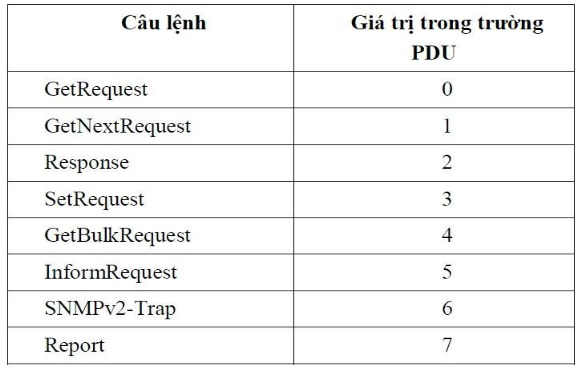
\includegraphics[scale=1]{images/snmpv2_2.jpg}\\
	Bảng thông tin trong trường PDU
\end{center}

- \textbf{Phiên bản SNMPv3}: SNMPv3 dựa trên việc thực hiện giao thức, loại dữ liệu và uỷ quyền như SNMPv2 và cải tiến phần an toàn. SNMPv3 cung cấp an toàn truy nhập vào các thiết bị bằng cách kết hợp sự xác nhận và mã khoá các gói tin trên mạng. 

Những đặc điểm bảo mật cung cấp trong SNMPv3 là:

+ Tính toàn vẹn thông tin: Đảm bảo các gói tin không bị sửa trong khi truyền. 

+ Sự xác nhận: Xác nhận nguồn của thông tin gửi đến. 

+ Mã khoá: Đảo nội dung của gói tin, ngăn cản việc gửi thông báo từ nguồn không được xác nhận. 

Tuy nhiên việc sử dụng SNMPv3 rất phức tạp và cồng kềnh dù nó là sự lựa chọn tốt nhất cho vấn đề bảo mật của mạng. Việc sử dụng sẽ tốn rất nhiều tài nguyên do trong mỗi bản tin truyền đi sẽ có phần mã hóa BER. Phần mã hóa này sẽ chiếm một phần băng thông đường truyền do đó làm tăng phí tổn mạng. Mặc dù được coi là phiên bản đề nghị cuối cùng và được coi là đầy đủ nhất nhưng SNMPv3 vẫn chỉ là tiêu chuẩn dự thảo và vẫn đang được nghiên cứu hoàn thiện. 

Khuôn dạng bảng tin SNMPv3: RFC 2572 định nghĩa các khuôn dạng bản tin SNMPv3. Khuôn dạng bản tin SNMPv3 được phân chia trong trong bốn phần Dữ liệu chung (Common data) - Trường này xuất hiện trong tất cả các bản tin SNMPv3. 

Bảo mật mô hình dữ liệu (Security model data) - Vùng này có ba phần: phần chung, phần dành cho sự chứng thực và phần cho dữ liệu riêng. 

Context – Hai trường nhận dạng và tên được dùng để cung cấp context cho PDU nào sẽ phải xử lý. 

PDU – Vùng này chứa một SNMPv2c PDU. 

\subsection{Các thành phần chính của giao thức SNMP}
Theo RFC1157, kiến trúc của SNMP bao gồm 2 thành phần: các trạm quản lý mạng (Network Management Station) và các thành tố mạng (Network Element). Network Management Station thường là một máy tính chạy phần mềm quản lý SNMP (SNMP management application), dùng để giám sát và điều khiển tập trung các network element.
\subsection{Kiến trúc giao thức SNMP}

 Giao tiếp giữa management và element:
\begin{center}
	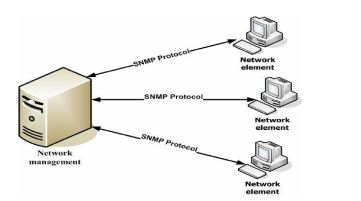
\includegraphics[scale=1]{images/kientrucsnmp.jpg}
\end{center}
Kiến trúc của SNMP bao gồm 2 thành phần:

- Các trạm quản lý mạng (network management station) : thường là một máy tính chạy phần mềm quản lý SNMP. Nhiệm vụ dùng để giám sát và điều khiển tập trung các network element.

- Các thành tố mạng(network element): device, host và application.

- SNMP agent: là một tiến trình (process) chạy trển network element. Nhiệm vụ cung cấp thông tin của element cho station, nhờ đó station có thể quản lý element.

{\bf Chú ý:} 

+ Một mangagement station có thể quản lý nhiều element, một 

+ Nếu 2 station tác động đến cùng một element thì element sẽ đáp ứng 2 tác động theo thứ tự cái nào đến trước sẽ xử lí trước.

\subsection{Quản lý giao tiếp trong SNMP}

Hệ thống quản lý mạng dựa trên SNMP gồm ba thành phần: bộ phận quản lý (manager), thiết bịchịu sự quản lý – còn gọi là đại lý (agent) và cơ sởdữ liệu gọi là Cơ sở thông tin quản lý (MIB). Mặc dù SNMP là một giao thức quản lý việc chuyển giao thông tin giữa ba thực thể trên, song nó cũng định nghĩa mối quan hệ client-server (chủ tớ). Cơ sở dữ liệu do agent SNMP quản lý là đại diện cho MIB của SNMP. Minh họa mối quan hệ giữa ba thành phần SNMP này.

\begin{center}
	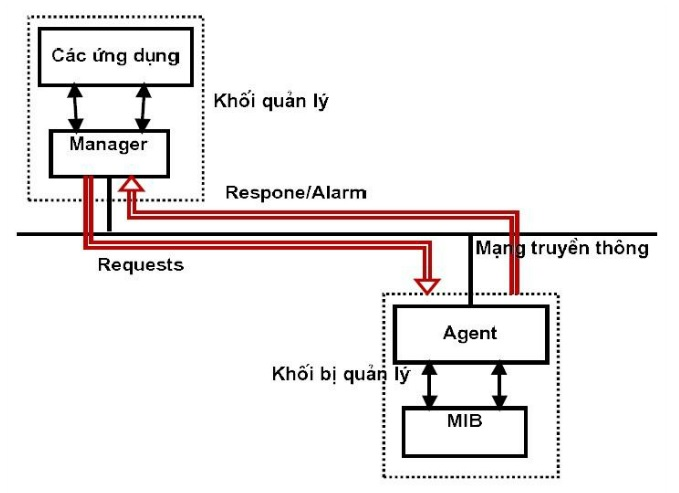
\includegraphics[scale=0.8]{images/giaotiepsnmp.jpg}\\
	Mối quan hệ giữa các thành phần SNMP
\end{center}

\subsubsection{Bộ phận quản lý (manager)} 

Bộ phận quản lý là một chương trình vận hành trên một hoặc nhiều máy tính trạm. 

Tùy thuộc vào cấu hình, mỗi bộ phận quản lý có thể được dùng để quản lý một mạng con, hoặc nhiều bộ phận quản lý có thể được dùng để quản lý cùng một mạng con hay một mạng chung. Tương tác thực sự giữa một người sử dụng cuối (end-user) và bộ phận quản lý được duy trì qua việc sử dụng một hoặc nhiều chương trình ứng dụng mà, cùng với bộ phận quản lý, biến mặt bằng phần cứng thành trạm quản lý mạng (NMS). Ngày nay, trong thời kỳ các chương trình giao diện người sử dụng đồ họa (GUI), hầu hết những chương trình ứng dụng sẽ cho ra giao diện sử dụng con trỏ và chuột để phối hợp hoạt động với bộ phận quản lý tạo ra những bản đồ họa và biểu đồ cung cấp những tổng kết hoạt động của mạng dưới dạng thấy được. Qua bộ phận quản lý, những yêu cầu được chuyển tới một hoặc nhiều thiết bị chịu sự quản lý ban đầu SNMP được phát triển để sử dụng trên mạng TCP/IP và những mạng này tiếp tục làm mạng vận chuyển cho phần lớn các sản phẩm quản lý mạng dựa trên SNMP. Tuy nhiên SNMP cũng có thể được chuyển qua NetWare IPX và những cơ cấu vận chuyển khác.

\subsubsection{Agent}

Thiết bị chịu sự quản lý (Agent) là một nút mạng hỗ trợ giao thức SNMP và thuộc về mạng bịquản lý. Thiết bị có nhiệm vụ thu thập thông tin quản lý và lưu trữ để phục vụ cho hệ thống quản lý mạng. Những thiết bị chịu sự quản lý, đôi khi được gọi là những phần tử mạng, có thể là các bộ định tuyến và máy chủ truy nhập (Access Server), switch, bridge, hub và máy tính hay là máy in trong mạng. Mỗi thiết bị chịu sự quản lý bao gồm phần mềm hoặc phần sụn (firmware) dưới dạng mã phiên dịch những yêu cầu SNMP và đáp ứng của những yêu cầu đó. Phần mềm hoặc phần sụn này được coi là một agent. Mặc dù mỗi thiết bị bắt buộc bao gồm một agent chịu quản lý trực tiếp, những thiết bị không tương thích với SNMP cũng có thể quản lý được nếu như chúng hỗ trợ một giao thức quản lý độc quyền. Để thực hiện được điều này phải có agent ủy nhiệm (proxy agent). Proxy agent này có thể được coi như một bộ chuyển đổi giao thức vì nó phiên dịch những yêu cầu SNMP thành giao thức quản lý độc quyền của thiết bị không hoạt động theo giao thức SNMP. Mặc dù SNMP chủ yếu là giao thức đáp ứng thăm dò (poll-respond) với những yêu cầu do bộ phận quản lý tạo ra dẫn đến những đáp ứng trong agent, agent cũng có khả năng đề xướng ra một “đáp ứng tự nguyện”. Đáp ứng tự nguyện này là điều kiện cảnh báo từ việc giám sát agent với hoạt động đã được định nghĩa trước và đáp ứng này cảnh báo việc agent đã tới ngưỡng định trước. Dưới sự điều khiển SNMP, việc truyền cảnh báo này được gọi là cái bẫy (TRAP).

\subsubsection{Cơ sở thông tin quản lý – MIB}

Mỗi thiết bị chịu sự quản lý có thể có cấu hình, trạng thái và thông tin thống kê định nghĩa chức năng và khả năng vận hành của thiết bị. Thông tin này rất đa dạng, có thể bao gồm việc thiết lập chuyển mạch phần cứng, những giá trị khác nhau lưu trữ trong các bảng ghi nhớ dữ liệu, bộ hồ sơ hoặc các trường thông tin trong hồ sơ lưu trữ ở các file và những biến hoặc thành phần dữ liệu tương tự. Nhìn chung, những thành phần dữ liệu này được coi là Cơ sở thông tin quản lý của thiết bị chịu sự quản lý. Xét riêng, mỗi thành phần dữ liệu biến đổi được coi là một đối tượng bị quản lý và bao gồm tên, một hoặc nhiều thuộc tính và một tập các hoạt động (operation) thực hiện trên đối tượng đó. Vì vậy MIB định nghĩa loại thông tin có thể khôi phục từ một thiết bị chịu sự quản lý và cách cài đặt thiết bị mà hệ thống quản lý điều khiển. 

\begin{center}
	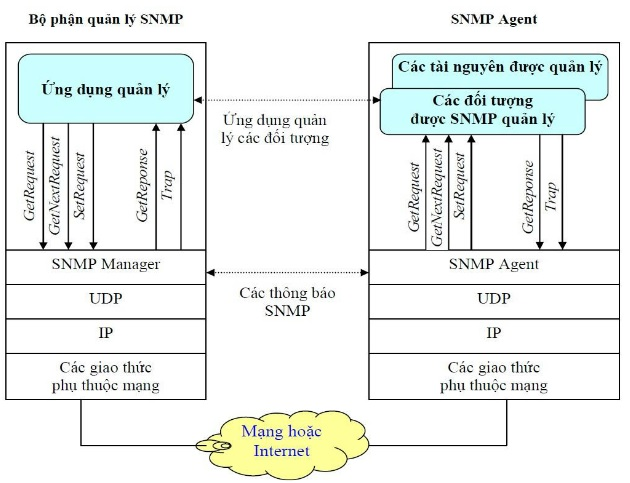
\includegraphics[scale=0.8]{images/giaotiepsnmp2.jpg}\\
	Mô hình giao thức hoạt động SNMP
\end{center}

\begin{center}
	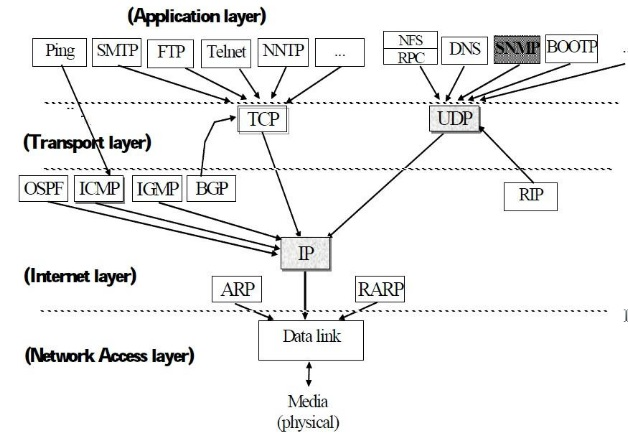
\includegraphics[scale=0.8]{images/giaotiepsnmp3.jpg}\\
	Vị trí của SNMP trong chồng giao thức TCP/IP
\end{center}

\subsection{Các cơ chế bảo mật trong SNMP}
Cơ chế bảo mật đơn giản gồm có: community string, view và SNMP access control list.

{\it Community string}: là một chuỗi ký tự được cài đặt giống nhau trên cả SNMP manager và SNMP agent, đóng vai trò như "mật khẩu" giữa 2 bên khi trao đổi giữa liêu. Community string có 3 loại: Read-community, Write-Community và Trap-Community. Khi agent nhận được bản tin request thì nó sẽ so sánh Read-community do manager gửi và Read-community mà được cài đặt. Nếu 2 chuỗi này giống nhau, agent sẽ trả lời; còn nếu không thì agent sẽ không trả lời.

{\it View}: Khi manager có read-community thì nó đọc toàn bộ OID của agent. Tuy nhiên agent quy định chỉ cho phép đọc một số OID có liên quan nhau- một phần của MIB. Tập con này gọi là view.

{\it SNMP access control list}: SNMP ACL là một danh sách các địa chỉ IP được phép quản lý/giám sát agent, nó chỉ áp dụng riêng cho giao thức SNMP và được cài trên agent. Nếu một manager có IP không được phép trong ACL gửi request thì agent sẽ không xử lý, dù request có community string là đúng. Đa số các thiết bị tương thích SNMP đều cho phép thiết lập SNMP ACL.
\chapter{CÔNG CỤ GIÁM SÁT MẠNG CACTI}
\section{Giới thiệu về công cụ giám sát mạng Cacti}
Sự phát triển của các thiết bị phần cứng mạng như : máy tính cá nhân, máy chủ, thiết bị định tuyến, Switch, Hub, \ldots và các dịch vụ mạng truyển file FTP, VPN, MAIL, \ldots đòi hỏi lớn hơn về băng thông mạng.

Quản lý mạng có thể xem như quản lý tất cả các tài nguyên mạng nhằm duy trì và đảm bảo sự ổn định của toàn bộ hệ thống mạng, đảm bảo an toàn thông tin trên mạng và mở rộng mạng. Hiện nay có rất nhiều phần mềm quản lý hệ thống tài nguyên mạng sử dụng thiết bị phần cứng đắt tiền. Tuy nhiên một số phần mềm nguồn mở cũng đáp ứng một cách toàn diện với nhiều tính năng linh hoat vượt trội. Với các phần mềm CACTI có khả năng bổ sung nhiều chương trình plugins giúp giải quyết được toàn bộ những khó khăn của doanh nghiệp trong việc quản lý tài nguyên, cho phép quản lý sự cố, quản lý topo mạng và cấu hình thiết bị mạng. Tất cả tạo nên một hệ thống mạng chủ động. 
\section{Kiến trúc phần mềm Cacti}
\section{Cài đặt Cacti trên Windows}
\section{Triển khai và ứng dụng Cacti trong giám sát mạng}
\subsection{Mô hình triển khai}
\subsection{Cấu hình Cacti}

\newpage
\vspace*{0.2cm}
\centerline{\Large\bf KẾT LUẬN CHUNG}
\vspace*{0.5cm}
\addcontentsline{toc}{chapter}{\bf KẾT LUẬN CHUNG}

\newpage
\vspace*{0.2cm}
\centerline{\Large\bf TÀI LIỆU THAM KHẢO}
\vspace*{0.5cm}
\addcontentsline{toc}{chapter}{\bf TÀI LIỆU THAM KHẢO}

%\bibliographystyle{ksfh_nat}
%	\bibliography{references} % expects file "references.bib"
\begin{enumerate}
\item Wikipedia, "Simple Network Management Protocol",

https://en.wikipedia.org/wiki/SNMP
\item{Wikipedia, "Network monitoring",

https://en.wikipedia.org/wiki/Network\_monitoring}
\item{TBT - VNCERT, "Tổng quan về hệ thống giám sát mạng",

http://www.vncert.gov.vn/}
\item{Diệp Thanh Nguyên, "SNMP Toàn tập", 04/2010

https://sites.google.com/site/snmptoantap/home}
\item "Complete List of Cacti Scripts and Templates", topic 15067, Cacti Official Forums and Support.
\end{enumerate}
	
\end{large}		

\end{document}